%%% Fiktivní kapitola s ukázkami sazby

\chapter{Analýza}

V této kapitole je detailně popsán problém a způsoby jeho navrženého a současného řešení. Dále zdroje dat se kterými budeme v této práci pracovat.

\section{Úvod}

Spoje které zajišťují hromadnou dopravu jezdí podle jízdních řádů, které definují jejich trasu. Trasa se udává sekvencí projíždících zastávek, časy příjezdu a odjezdu do, resp. z těchto zastávek a vzdáleností zastávek od výchozího bodu spoje. Tyto zastávky jsou zpravidla jediné refenční body u kterých je možno zjistit skutečné zpoždění, nebo předjetí (dále uvažováno jako zpoždění se zápornou hodnotou). Dále jsou součástí jízdních řádů také velice detailní nákresy tras každého spoje, formou lomené čáry definovanou posloupností souřadnic, kde každý bod je doplněn o jeho vzdálenost od výchozího bodu spoje.

\bigbreak

Délka trasy mezi dvěma refernčními body nezříka dosahuje i několika desítek kilometrů\footnote{Podle dat pro spoje jedoucí v 20. 2. 2020 je medián vzdálesnotí mezi zastávkama, mezi kterýma projede alesponˇ jeden spoj denně 943 m. Průjezdů mezi zatávkami ve vzdálenosti více než 10 kilometrů je 784, přiřičemž průjezdů mezi zastávkami ve vzdálenosti alesponˇ 2 km je přibližně 15000}. Na těchto úsecích mohou vznikat mimořáné události, které se dají predikovat jen s těží. Nicméně ve většině případů je průběh jízdy ovlivněn pouze obvyklým provozem v dané denní době.

Detailní rozbor počtu průjezdů mezi zastávkami v daných vzdálenostech je vidět na grafu \ref{fig:stop_distances_result}. Kde průjezdem se myslí každý jednotlivý průjezd vozidla mezi danou dvojcí zastávek v daný den. Data jsou platná pro spoje jedoucí v 20. 2. 2020.

\begin{figure}
	\centering
  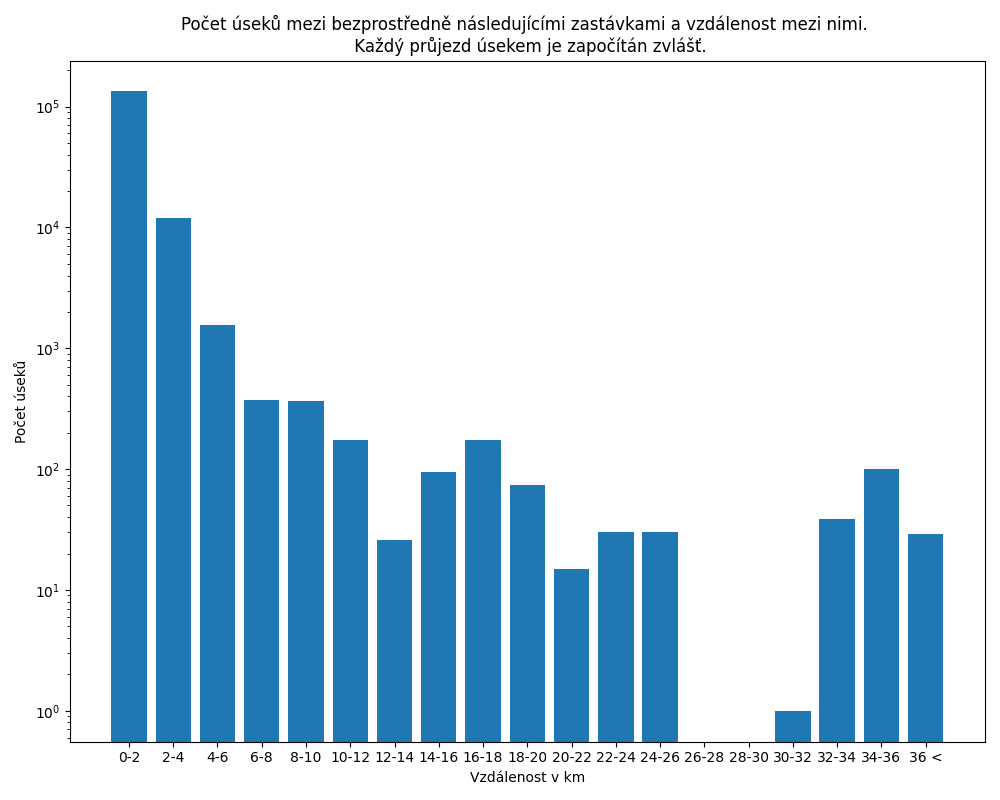
\includegraphics[width=0.6\linewidth]{../img/stop_distances_plot_2020-02-20.png}
  \caption{Graf počtu úseků mezi následujícími zastávkami a vzdálenotí mezi nimi.}
  \label{fig:stop_distances_result}
\end{figure}

\section{Popis problému odhadu zpoždění}

Řešený problém se týká případu, kdy vozidlo projíždí mezi dvěma referenčními body a tato trasa má části, ve kterých vozidlo jede různou rychlostí. Např. vozidlo při vyjíždění z města jede mnohem pomaleji než při jízdě mezi městy. Takových úseků, na kterých se rychlost jízdy liší může být na trase více a nedají se všechny jednoduše detekovat.

\bigbreak

Tato Práce tedy modeluje profily jízd mezi referenčními body. A na základě toho zpřesnit odhad zpoždění. Tento odhad by měl být mnohem přesnější než současné odhady, které odpovídají tomu, že vozidlo jede konstantní rychlostí po celou dobu jízdy. Nebo je takové možné brát jako aktuální zpoždění spoje poslední změřené zpoždění při průjezdu nějakých referenčním bodem (zastávkou, nebo např. pro tramvaje se používají návěstidla).

\bigbreak

Přidaná hodnota je tedy v tom, že Práce navrhne takové modely, které nebudou penezalizovat zvyšováním zpožděním za pomalou jízdu v úsecích, které se pomaleji projždějí vždy. A také naopak zvýhodnˇovat snížením zpožděním za rychlou jízdu v úsecích, které se projíždějí rychle. Pokud bychom se tedy podívali na změny zpoždění na trase mezi dvěma referečními body, v ideálním případně by měli být nulové.

\bigbreak

Pro řešení odhadu toho typu spoždění stačí navrhnout systém na odhat zpoždění v půběhu jízdy mezi referenčními body z historikých dat jízd.

\bigbreak

Pro vyloučení všech pochybností je hodno uvést, že se naše Práce nesnaží předpovědět zpoždění, které spoj může nabrat vzhledem k dosavadnímu průběhu trasy. Tedy např. nijak nezohlednˇuje to, že spoj právě stojí v mimořádné koloně a dalo by se tedy předpokládat, že zpoždění bude rychle růst i v následujících minutách. Ale naopak Práce se snaží odhadnou zpoždění v danném bodě na trase vzhledem k obvyklému profilu jízdy. Tedy např. pokud by výše uvažavaná kolona byla pravidelná Práce ji zohlední ve statistických modelech.


\subsection{Příklad nelineárního profilu trasy} \label{subsection:priklad_nelinearni_trasa}

Celé ilustrováno na příkladě jízd mezi dvěma zastávkama K letišti a ZLičín, kde je nelineární profil jízdy vidět velice dobře. Jedná se totiž o trasu přesně odpovídající popisu problému.

\bigbreak

Popsané rozdíly v rychlosti a nelineární profil trasy je patrný na grafu \ref{fig:k_letisti_to_zlicin_3d}. Za povšimnutí táké stojí viditelné spomalení průjezdů v ranní špičce, 7--9 \footnote{časy jsou v UTC} hodina ráno.

\bigbreak

Tento příklad dále podrobněji analyzován v kapitole \ref{subsubsection:analyza_dat}.

\begin{figure}
  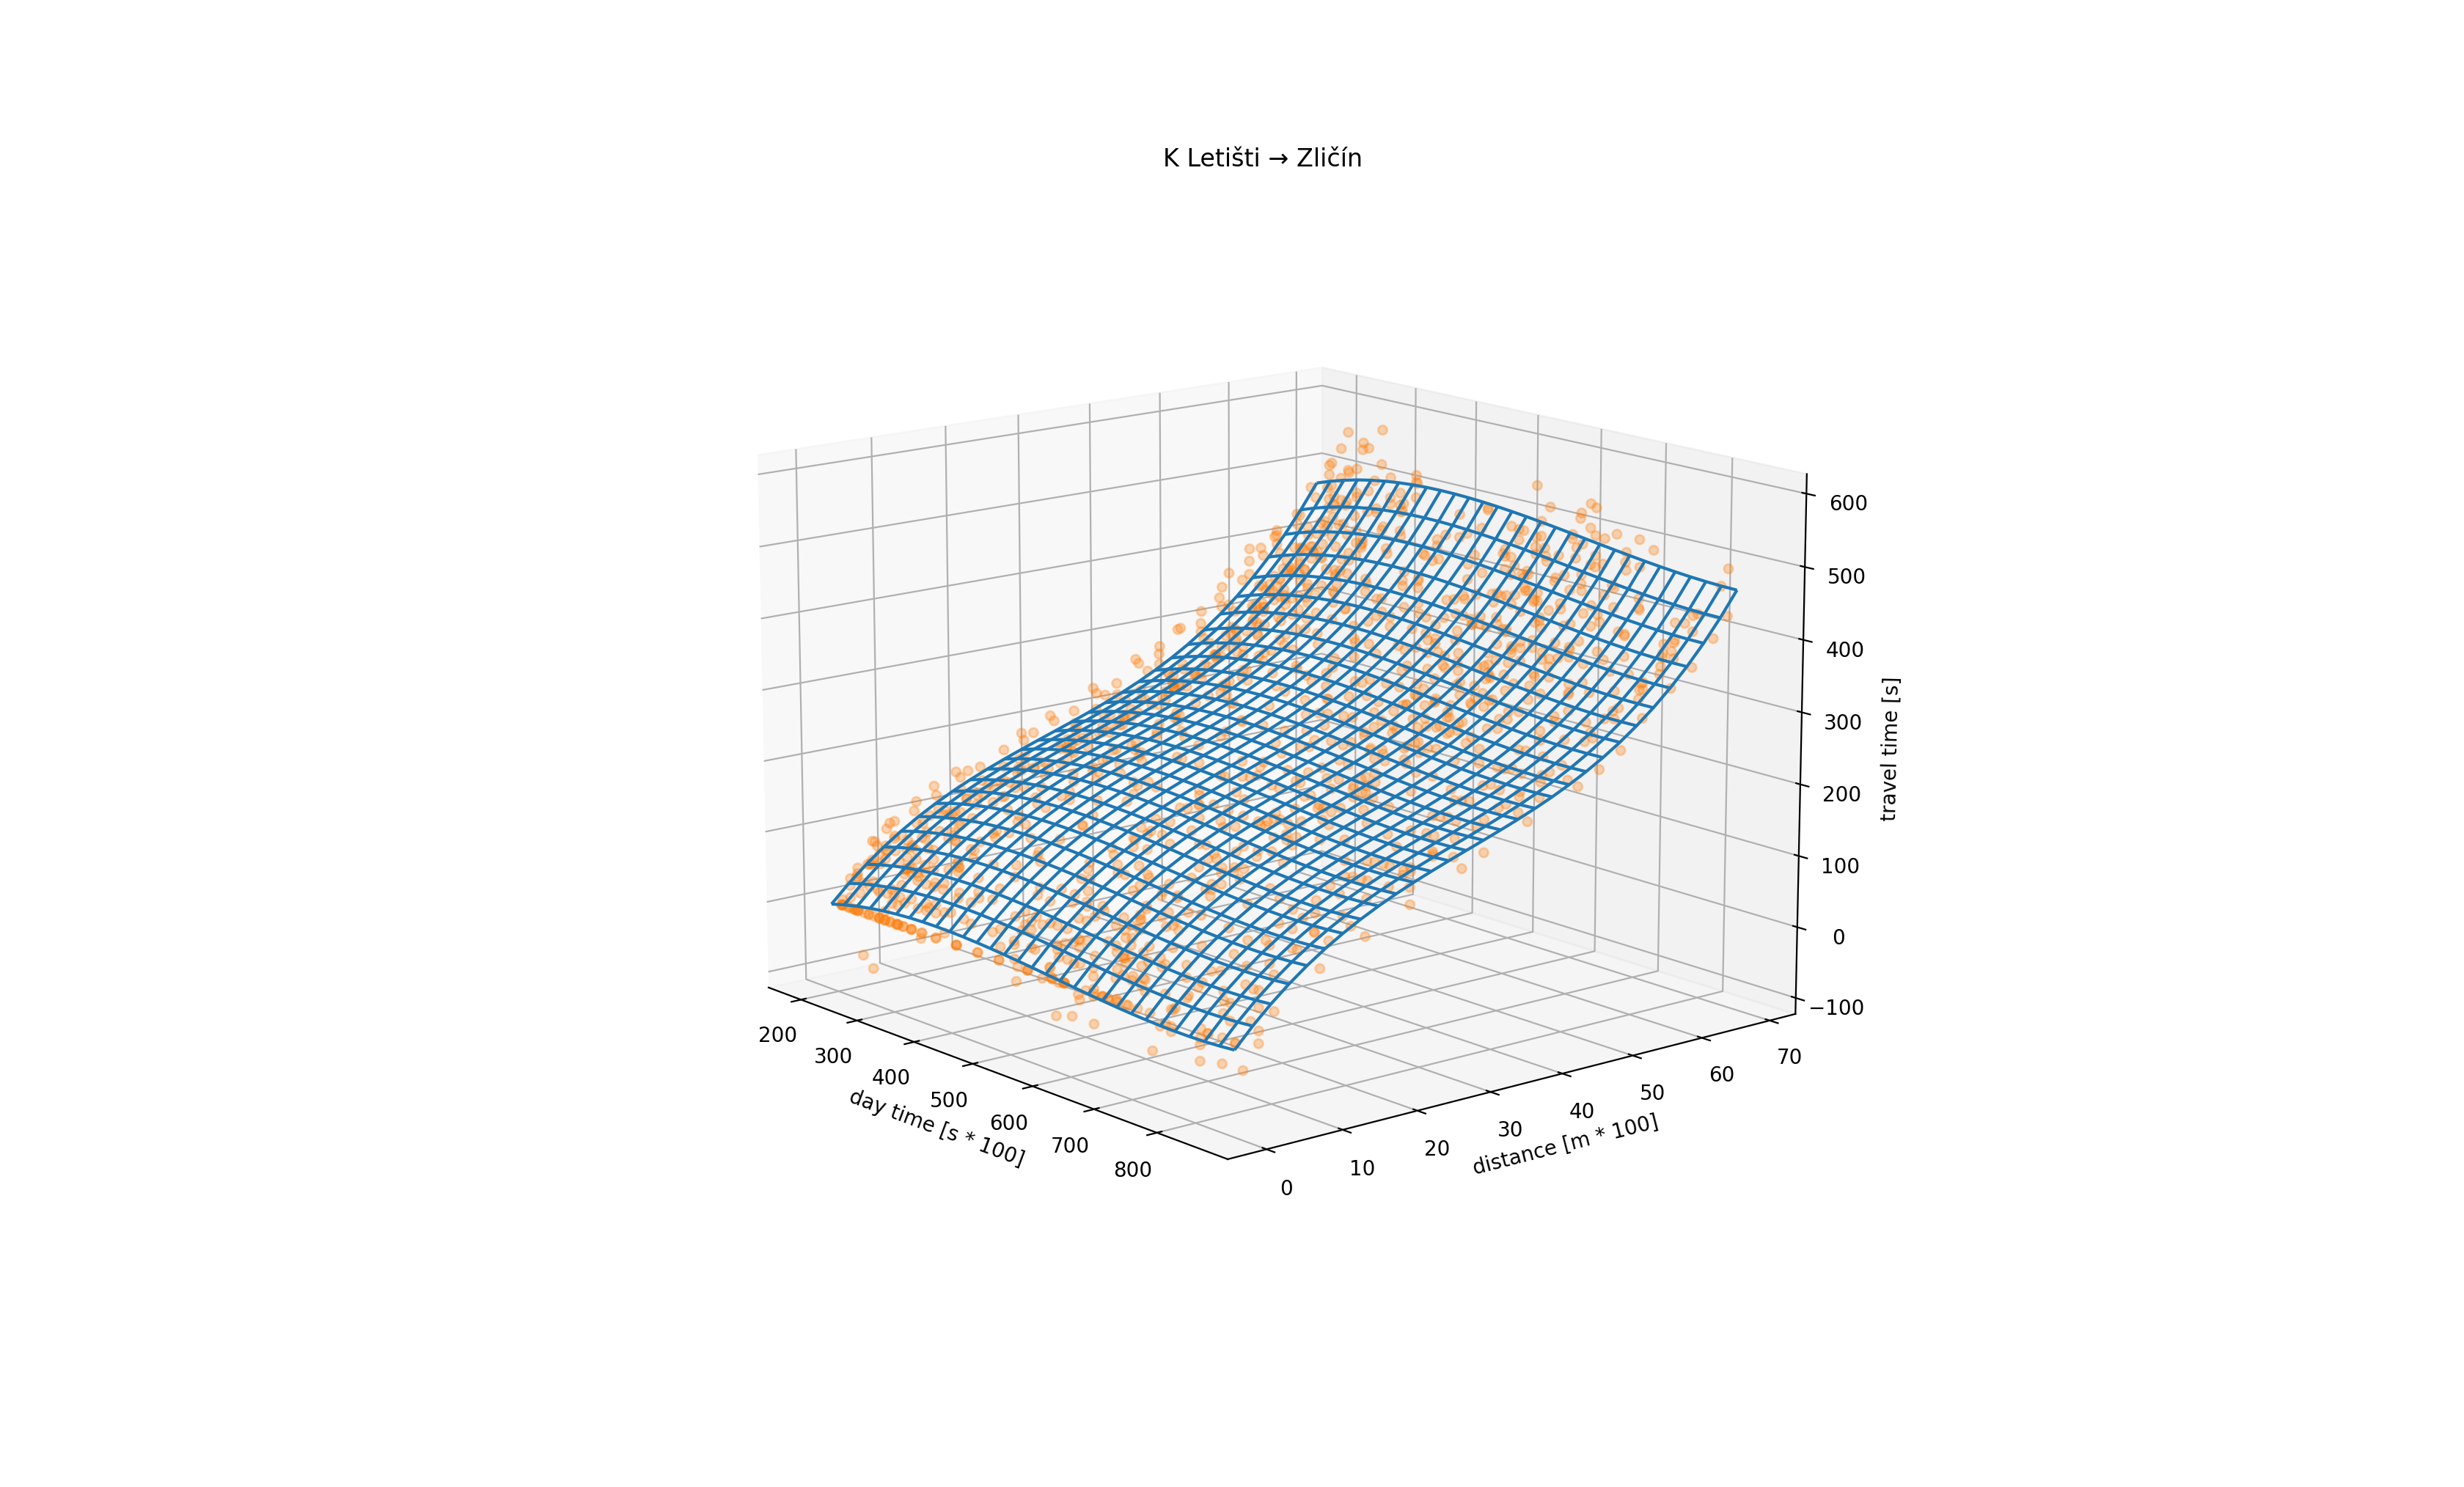
\includegraphics[width=\linewidth]{../img/k_letisti_to_zlicin_3d.png}
  \caption{Modrá plocha značí vymodelovaný profil trasy. Oražové body jsou jednotlivé vzorky polohy vozidel. Data pro graf jsou ze dnů 20.--21. 2. 2020}
  \label{fig:k_letisti_to_zlicin_3d}
\end{figure}

\bigbreak

Na obrázku \ref{fig:k_letisti_to_zlicin_map} je pro bližší představu popsané trasy vidět trasa spoje vykreslená do mapy.

\begin{figure}
	\centering
  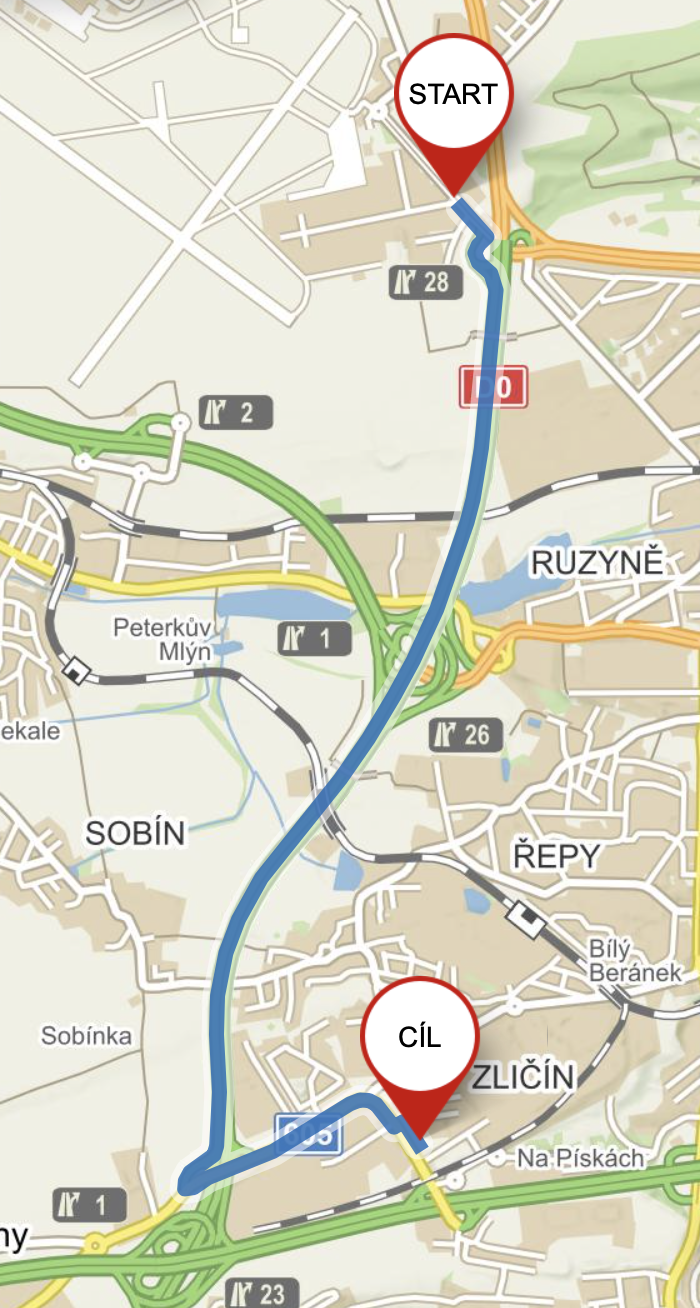
\includegraphics[width=0.3\linewidth]{../img/k_letisti_to_zlicin_map.png}
  \caption{Trasa mezi zastávkama K Letišti a Zličín. Zdroj: mapy.cz}
  \label{fig:k_letisti_to_zlicin_map}
\end{figure}

\subsubsection{Rozbor trasy}

Celá tato trasa má necelých 7 km a její průjezd spojem VHD trvá 10 minut. Prvních 600 metrů je vedeno po obecní komunikaci, přes křižovatku a nájezd na Pražský okruh. Průměrná rychlost vozidel byla 35 km/h\footnote{Počítáno podle vozidel, které poslaly polohu v 600m (resp. 4.9km, resp. 6.6km pro další údaje o rychlosti) vzdálenosti od zastávky. Počet záznamů o poloze vozidel se v různých vzdálenostech liší.}.

\bigbreak

Dále trasa pokračuje přes Pražský okruh rovně až do vzdálenosti 4.9 km od zastávky K Letišti, kde začíná nájezd na ulici Na Radost. Dá se předpokládat, že vozidla se na komunikaci vyšší třídy pohybují rychleji což dokazuje, že na tomto úseku trasy se průměrná rychlost vozidel zvýšila na 63 km/h.

\bigbreak

Poslední úsek se tedy skládá z výjezdu z Pražského okruhu, průjezdu křižovatkou, jízdy po obecní komunikaci a vjezdu do stanice Zličín. Délka úseku je 2 km. Průměrná rychlost za celou trasu se na tomto úseku snížila na 55 km/h.


\subsection{Současná řešení}

Algoritmus na odhat aktuálního zpoždění mezi dvěma referenčními body již exituje a je součástí Datové Platformy -- Golemio, ze kterého se čerpají data pro tuto práci. (Detailní popis dat uveden v kapitole ~\ref{chapter:TODO later}.)

\bigbreak

Nicméně tento algoritmus nijak nezohledňuje variabilitu profilu trasy. Totiž v tomto řešení je nahlíženo na postup vozidla na trase jako na lineární funkci vůči času. Je ovšem zřejmé, že rychlost vozidel není konstantní, neboli doba jízdy není linárně závislá na ujeté vzdálenosti.

\bigbreak

Proto je potřeba tento odhad zpřesnit, což je cílem naší práce. K tomuto cíli jsme byli nasměrování v rámci schůzky s pracvoníky společnosti OICT, kde bylo řečeno, že toto je problém současného řešení, který je potřeba vyřešit.



\section{Analýza zdroje dat} \label{section:analyza_zdroje}

V této kapitole je popsán zdroj real-timových dat o polohách vozidel využívané v této práci.

\subsection{Přístup k datům}

Vozidla vysílají data o své poleze při různých událostech. Zejména pak při brždění, rozjezdu, vyhlášení zastávky, nebo jinak každých 20 sekund\footnote{Řečeno zaměstnancem OICT na schůzce 4. 5. 2019}.

\bigbreak

Taková data pak přímo putují k provozavoateli systému na monitorování vozidel, kterým je společnost \gls{kapsch} jakožto partner \gls{dpp}. Ten však tato data zpracovává a posílá ke zveřejnění na platformě Golemio. Bohužel při tomto procesu zpracování se vytratí informace o události v jáké byly data pořízeny. Tedy informace o příjezdu nebo odjezdu ze zastávky jsou zjistitelné pouze z \gls{gps} souřadnic a následném odhadu pozice vozidla na trase dané linky.

\bigbreak

Po té co jsou tyto data přeneseny do společnosti Operátor ICT by měla být zveřejněna, nicméně data ve výše popsané podobě jsou poměrně chudá, proto je k nim přidáno více atributů. Jedná se o dopočet poslední projeté zastávky, ujeté vzdálenosti od výchozí stanice, zpoždění v poslední zastávce.

\bigbreak

 Z pohledu této práce je nejzajímavější informace o vzdálenosti, kterou vozidlo urazilo od jeho výchozí zastávky. Dále jsou přidána data o jízdních řádech a zastávkách jejichž původcem je \gls{ropid}.

\bigbreak

Real-time data o polohách, která jsou již neplatná (zastaralá) se neposílají (posílá vždy pouze nejaktuálnší informace) a i z Datové platformy jsou data po pár minutách nenávratně smazány.

\subsubsection{Dokumentace}

Na úvod je nutné poznamenat, že datová platforma je stále ve vývoji a formát dat se může měnit. S tím mohou přicházet určité výpadky a problémy. K jednomu takovému výpadku došlu i při vývoji této práce, kdy po dobu 14 dnů platfomarma vůbec neodpovídala na dotazy nebo vracela prázdné datasety.

\bigbreak

Současně s využívanou verzí \gls{api}, je nasazená i pokročilejší \gls{api} ve verzi 2, které obsahuje více informací a je přehledněji upravena. Nicméně při zahájení vývoje této práce nebyla verze 2 k dispozici, proto jsou využívána data pouze ze starší verze.

\bigbreak

Oficiální uživatelská dokumentace datové platformy\footnote{Golemio: https://golemioapi.docs.apiary.io} je poměrně zastaralá sama o sobě tak, že aktuální sada parametrů jí neodpovídá a neobsahuje žádné popisy nebo vysvětlení dat. Proto vysvětlení jednotlivých atributů se zakládá na intuitivním pochopení nebo vyplynulo z jednání se správci platformy. V následujících kapitolách bude popsán formát dat, tak jak přichází ze zdroje. Ten se může od oficiálně vystavené dokumentace lišit. A také budou popsány pouze atributy využívané v této práci nebo zajímavé pro její budoucí rozvoj.

\bigbreak

Každá datová sada je exportována ve formátu \gls{geojson} pokud se jedná o geografická data, nebo jinak ve formátu \gls{json}. Přistupuje se k nim přes jednotné webové rozhraní pomocí \gls{http} požadavku daného \gls{url} adresou a jeho hlavičkou.

\bigbreak

Ačkoli se dokumentace tváří tak, že data jsou exportována ve formátech \gls{json} nebo \gls{geojson}, většinou formát dat není přesně podle specifikace těchto formátů. Například může být uveden atribut \verb"wheelchair_accessible", který je typu \verb"bool" a je nastaven na hodnotu \verb"True", nicmně podle specifikace se tyto hodnoty píší s malým písmenem\footnote{V průběhu tvorby této práce byla chyba opravena.}. Pro tuto práci to sice nepředstavuje komplikaci, protože tento atribut není potřeba, ale mohlo by se stát, že některé parsery \gls{json}u vyhodnotí řetězec jako nevalidní a skončí chybou.

\bigbreak

Celá datová platforma Golemio je pojatá jako Open Source projekt\footnote{Programátorská dokumentace je dostupná na https://operator-ict.gitlab.io/golemio/documentation/}. Tedy je možné její zdrojový ko'd vylepšit či opravit nebo také čtením ko'du detailně porozumnět jak zde popisované zpracování dat funguje. Avšak takový rozbor zdrojového ko'du je mimo rozsah této práce.

\subsubsection{Pozice vozidel}

Ze zveřejněných dat na této platformě jsou nejdůležijtější data pro tuto práci pozice vozidel. Jelikož se jedná o real-time data, data rychle zastarávají a je nutné je velmi často aktualizaovat.

\bigbreak

Využívané atributy jsou:

\begin{itemize}
	\item \documentationAtt{coordinates}{aktuální \gls{gps} souřadnice vozidla}

	\item \documentationAtt{origin\_timestamp}{čas zachycení pozice vozidla, v časovém pásmu \gls{utc}}

	\item \documentationAtt{gtfs\_trip\_id}{unikátní identifikátor tripu pro spárování s jízdním řádem}

	\item \documentationAtt{gtfs\_shape\_dist\_traveled}{vzdálenost vozidla uražená od začátku tripu v metrech}

	\item \documentationAtt{delay\_stop\_departure}{zpoždění zachycené při odjezdu z poslední projeté zastávky v sekundách}
\end{itemize}.

Příklad dat popisující aktuální polohu vozidla, na kterém je možno vidět strukturu dat i další atrubuty. Řada z nich je pro tuto práci zbytečná. Dále je možno si povšimnout atrubutu \documentationAtt{all\_positions}, který obsahuje všechny zaznamenané pozice daného vozdila na jeho aktuální trase, tento atribut je z důvodů objemu dat volitelný a pro tuto práci se nevyužívá.

\begin{code}[frame=none]
"geometry":{
  "coordinates":[14.91724,50.41881],
  "type":"Point"
},
"properties":{
  "trip":{
    "cis_agency_name":"ČSAD Česká Lípa",
	"cis_id":"260467",
	"cis_number":3008,
	"cis_order":2,
	"cis_parent_route_name":"467",
	"cis_real_agency_name":"ČSAD Česká Lípa",
	"cis_short_name":null,
	"cis_vehicle_registration_number":1073,
	"gtfs_route_id":"L467",
	"gtfs_route_short_name":"467",
	"gtfs_trip_id":"467_252_200105",
	"id":"2020-02-23T18:50:00Z_260467_467_3008",
	"start_cis_stop_id":30107,
	"start_cis_stop_platform_code":"A",
	"start_time":"19:50:00",
	"start_timestamp":"2020-02-23T18:50:00.000Z",
	"vehicle_type":4,
	"wheelchair_accessible":true
  },
  "last_position":{
    "bearing":20,
	"cis_last_stop_id":21393,
	"cis_last_stop_sequence":28,
	"delay":261,
	"delay_stop_arrival":null,
	"delay_stop_departure":287,
	"gtfs_last_stop_id":"U3389Z1",
	"gtfs_last_stop_sequence":30,
	"gtfs_next_stop_id":"U2987Z30",
	"gtfs_next_stop_sequence":31,
	"gtfs_shape_dist_traveled":"64.1",
	"is_canceled":false,
	"lat":"50.41881",
	"lng":"14.91724",
	"origin_time":"21:29:37",
	"origin_timestamp":"2020-02-23T20:29:37.000Z",
	"speed":20,
	"tracking":2,
	"trips_id":"2020-02-23T18:50:00Z_260467_467_3008"
	},
  "all_positions":{
    "features":[],
	"type":"FeatureCollection"
  }
},
"type":"Feature"

\end{code}

\subsubsection{Jízdy}

Dále jsou k dispozici data o každé jízdě. To je popis trasy vozidla, včetně zastávek a časů příjezdů a odjezdů do/z nich. Také může být vyžádáno k informacím o jízdě připojit celý shape trasy, tj. lomená čára kopírující celou trasu daného tripu po povrchu Země.

\bigbreak

 Míra unikátnosti identifikátorů těchto tripů je předmětem dohadů a zřejmě jsou pod správou plánovačů \gls{mhd}, nicméně pro účely této práce může být předpokládáno, že každá jízda má vlastní jízdní řád, který se váže na čas a každá jízda jede nejvýše jednou za den.

\begin{itemize}
	\item \documentationAtt{trip\_headsign}{nápis na čele vozidla, typicky cílová stanice}

	\item \documentationAtt{route\_id}{číslo linky}

	\item \documentationAtt{trip\_id}{unikátní identifikátor tripu pro spárování s real-time daty, pravděpodobně odpovídá atributu \verb"gtfs\_trip\_id"}


\end{itemize}

Navíc s každým tripem může být vyžádáno zaslání seznamu zastávek, kterýma projíždí. Zde jsou k dispozici informace vázající se k danému průjezdu zastávkou. Každá uvená zastávka s sebou nese i kompletní informaci o sobě, tedy má stejnou informační hodnotu jako samostatný dotaz na jednotlivé zastávky z datové sady zastávek.

\subsubsection{Zastávky}

\begin{itemize}
	\item \documentationAtt{arrival\_time}{čas příjezdu spoje do zastávky}

	\item \documentationAtt{departure\_time}{čas odjezdu spoje do zastávky}

	\item \documentationAtt{shape\_dist\_traveled}{vzdálenost zastávky na trase od výchozího bodu daného tripuv metrech}

	\item \documentationAtt{stop\_id}{unikátní indetifikátor zastávky}

	\item \documentationAtt{coordinates}{\gls{gps} souřadnice zastávky, často \verb"null", je třeba využít atributy \verb"stop\_lat" a \verb"stop\_lon"}

	\item \documentationAtt{stop\_name}{název zastávky}
\end{itemize}

\bigbreak

Příklad dat popisujících jednu jízdu včetně zastávek. Seznam zastávek a body trasy jsou zkráceny vzhledem k objemu dat.

\begin{code}[frame=none]
"bikes_allowed":2,
"block_id":"",
"direction_id":1,
"exceptional":1,
"route_id":"L421",
"service_id":"1111100-1",
"shape_id":"L421V4",
"trip_headsign":"Kolín,Nádraží",
"trip_id":"421_225_191114",
"trip_operation_type":1,
"trip_short_name":"",
"wheelchair_accessible":2,
"stop_times":[{
  "arrival_time":"14:14:00",
  "arrival_time_seconds":null,
  "departure_time":"14:14:00",
  "departure_time_seconds":null,
  "drop_off_type":"0",
  "pickup_type":"0",
  "shape_dist_traveled":0,
  "stop_headsign":"",
  "stop_id":"U2033Z5",
  "stop_sequence":1,
  "timepoint":null,
  "trip_id":"421_225_191114",
  "stop":{
    "geometry":{
      "coordinates":[
        null,
        null
      ],
      "type":"Point"
    },
    "properties":{
      "level_id":"",
      "location_type":0,
      "parent_station":"",
      "platform_code":"5",
      "stop_code":null,
      "stop_desc":null,
      "stop_id":"U2033Z5",
      "stop_lat":49.87486,
      "stop_lon":14.9078,
      "stop_name":"S\u00e1zava,Aut.st.",
      "stop_timezone":null,
      "stop_url":"",
      "wheelchair_boarding":0,
      "zone_id":"5"
    },
    "type":"Feature"
  },
  ...
],},
"shapes":[{
  "geometry":{
    "coordinates":[
      14.90778,
      49.87494
    ],
    "type":"Point"
  },
  "properties":{
    "shape_dist_traveled":0,
    "shape_id":"L421V4",
    "shape_pt_lat":49.87494,
    "shape_pt_lon":14.90778,
    "shape_pt_sequence":1
  },
  "type":"Feature"
},
...
]

\end{code}

\subsection{Analýza statických dat}

Sběr dat probíhal ve dnech 20.--24. 2. 2020.

\bigbreak

Data byla přebírána pouze z dat o každé jednotlivé jízdě a aktuálních poloh vozidel stahovaných každých 20 sekund. Tedy pokud určitou zastávkou žádný spoj neprojel nebo se uložení spoje z důvodu neúplných dat nezdařilo, může nějaká zastávka v databázi chybět. Stejně tak mohou chybět i nějaké spoje. Nejčastěji chybějící požadovaná data jsou informace o spoždění spoje v poslední zastávce, zcela nenalezený spoj ve zdroji dat a tedy chybějící jízdní řád. Nicméně jedná se zanedbatelné množství. Práce totiž nemůže počítat s poškozenými daty a není jejím úkolem držet všechny zastávky, ale pouze ty kterými nějaký spoj projíždí. To z důvodu přehlednosti zastávek při vizualizaci, kde ukazovat nepoužívané zastávky nemá smysl a také pro odhady zpoždění nedává smysl počítat něco pro zastávku, která není obsluhovaná.

\subsubsection{Zastávky} \label{subsubsection:zastavky}

Do databáze bylo celkem vloženo 5820 nástupištˇ, které náleží celkem 2961 zastávkám. Ale naprostá většina (74 \%) zastávek jsou párová, tedy mají pouze 2 nástupiště. Jednosměrných zastávek je 18 \%, zastávek se 3 nástupišti jsou 3 \%. Nejvíce nástupištˇ mají stanice Slaný Aut. nádr. (14), Černý Most (12), Kladno Autobusové nádraží (11).

\subsubsection{Jízdy}

Celkem bylo nalezeno 12788 spojů, z nich naprostá většina vyjela opakovaně v následující den\footnote{Ze všech vypravených jízd ve dnech 20. 2. 2020 (9334) a 21. 2. 2020 (9428) jich 9051 bylo označeno ve zdrojových datech stejným identifikátorem, tedy z našeho pohledu sdílely jízdní řád a cestu.}.

Další rozbor dat na grafu \ref{fig:stop_distances_result} a v kapitole \ref{TODO:statistika}.




\section{Analýza vizualizačních nástrojů}

Jak bylo řečeno v úvodu, součástí práce je i vizualizace spočítaných dat.

\bigbreak

To bude provedeno formou front endové aplikace, která zobrazuje mapu a do ní zanáší data o vozidlech VHD. Funkční požadavky této aplikace jsou inspirované již existujícími řešeními tohoto problému.

\subsection{Současná řešení} \label{subsection:soucasna_reseni_front_end}

Vizualizaci vozidel \gls{vhd} do mapy již nabízí několik portálů. Všechny jsou však poměrně strohé.

\subsubsection{Golemio}

Takovou mapu zobrazuje i samotný provozavatel datové platformy. Nicméně nejsou zde vidět ani čísla linek zobrazených autobusů, natož pak nějaké další informace. Příklad vizualizace je uveden na obrázku \ref{fig:golemio_result}.

\begin{figure}
  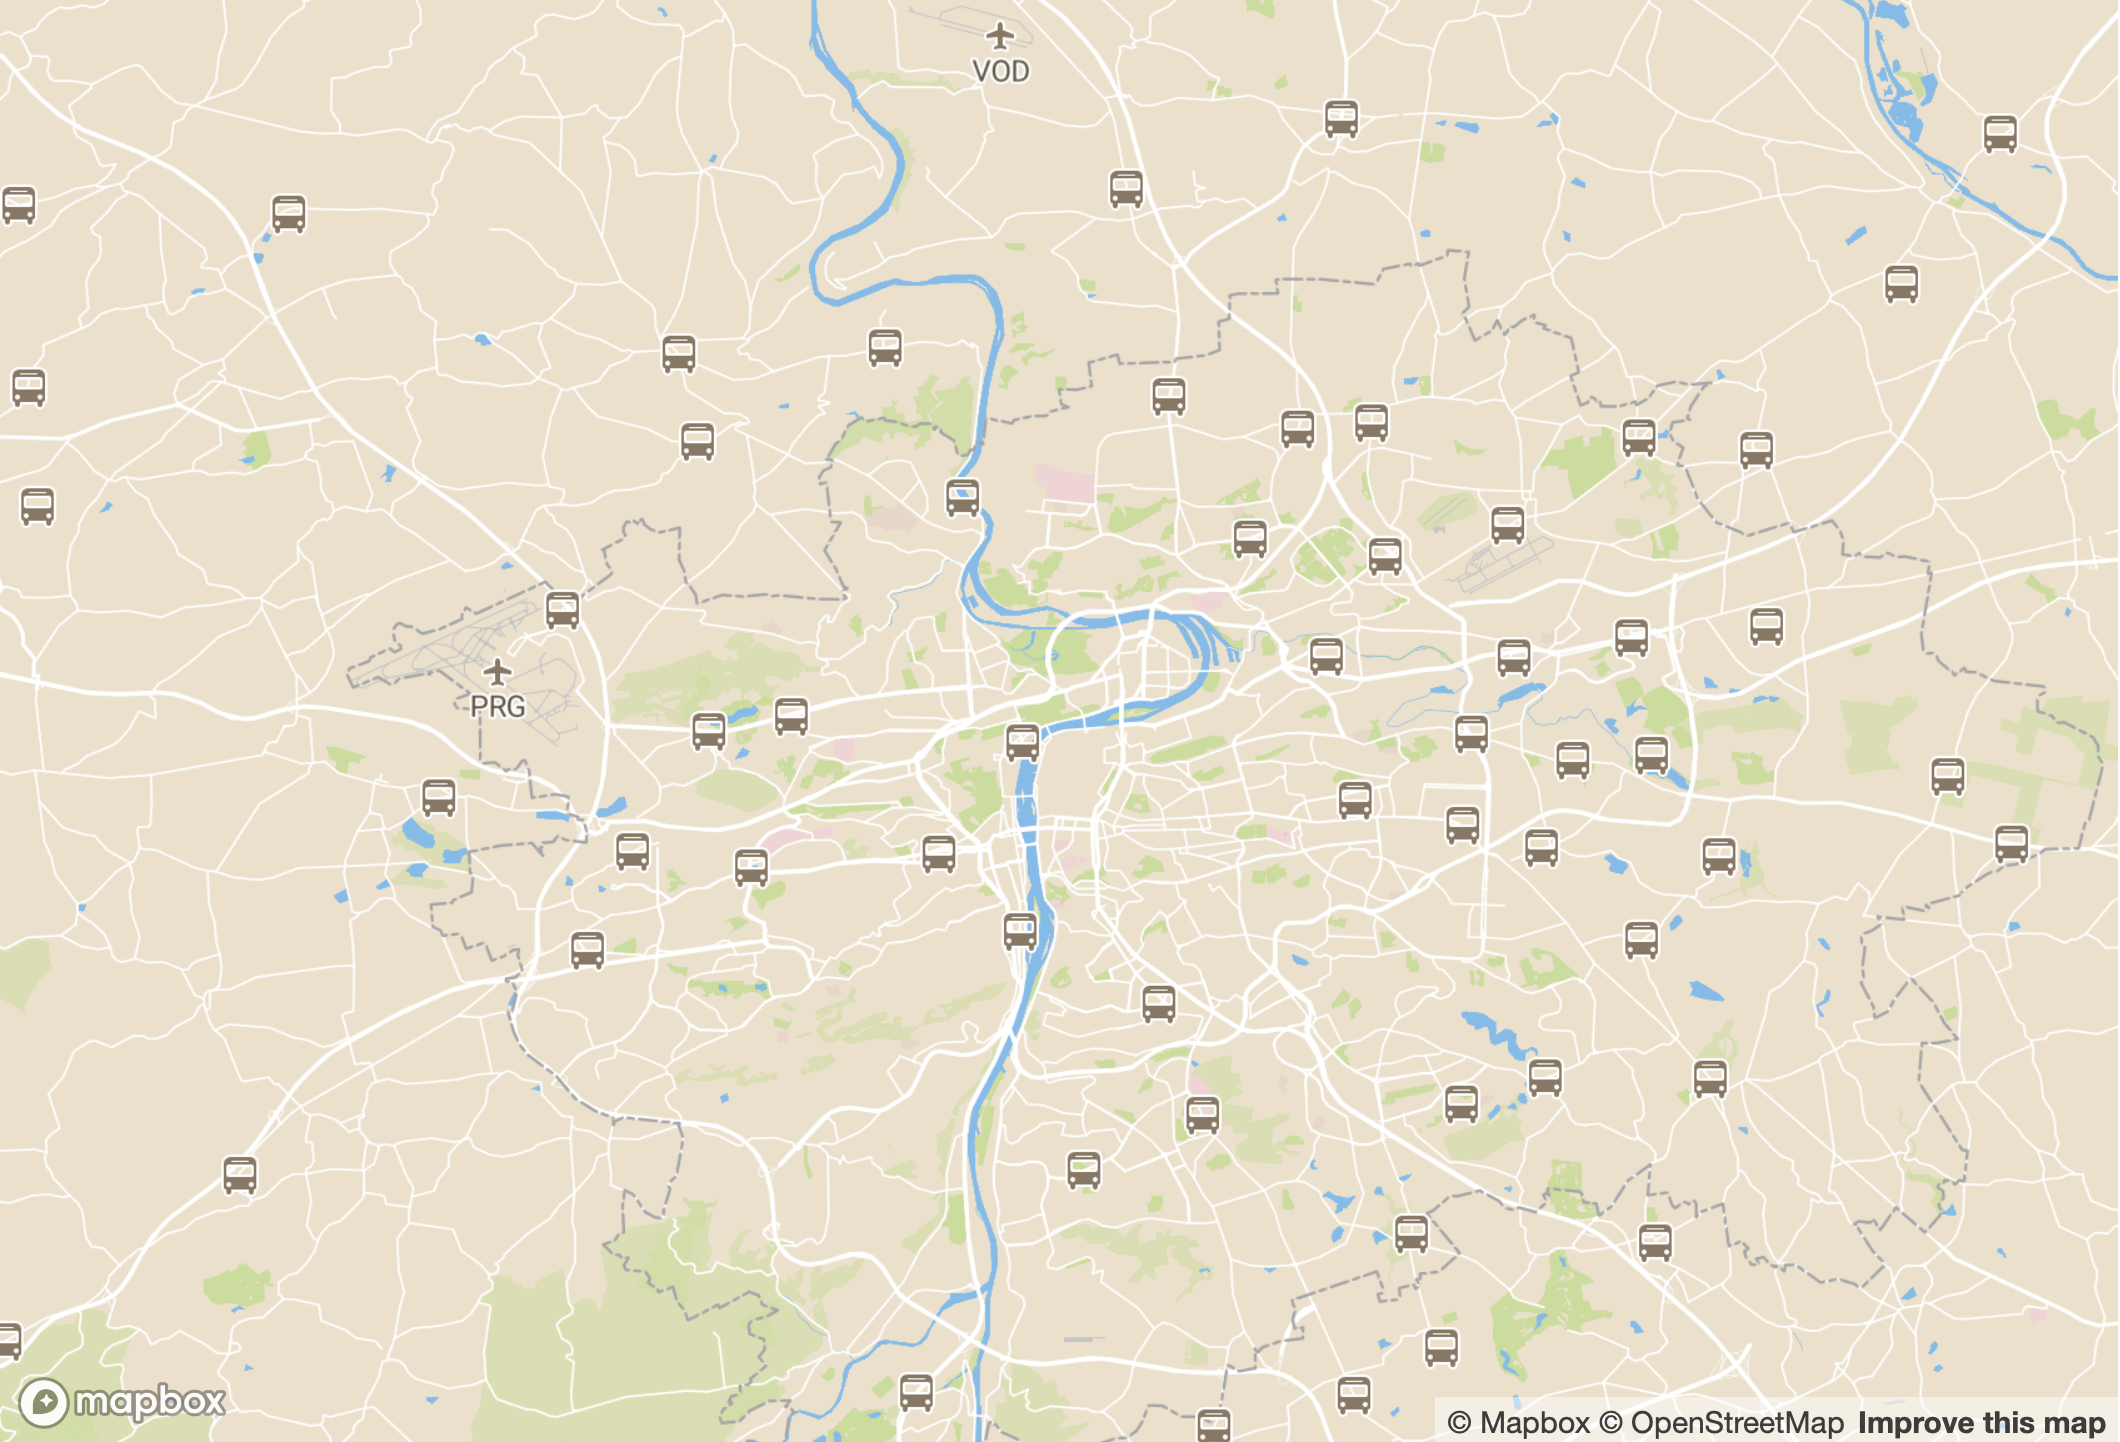
\includegraphics[width=\linewidth]{../img/golemio_mapa.png}
  \caption{Mapa z golemio.cz.}
  \label{fig:golemio_result}
\end{figure}

\subsubsection{Tram-bus}

Dalším poskytovatelem je portál tram-bus, který si vede o něco lépe. Ukazuje směr jízdy vozidel, čísla linek a po kliknutí informace o zpoždění a nejbližší zastávky. Pozn.: na mapě již jsou vidět spoje \gls{dpp}, protože v době psaní této práce již byly data veřejné. Příklad vizualizace je uveden na obrázku \ref{fig:tram-bus_result}.

\begin{figure}
  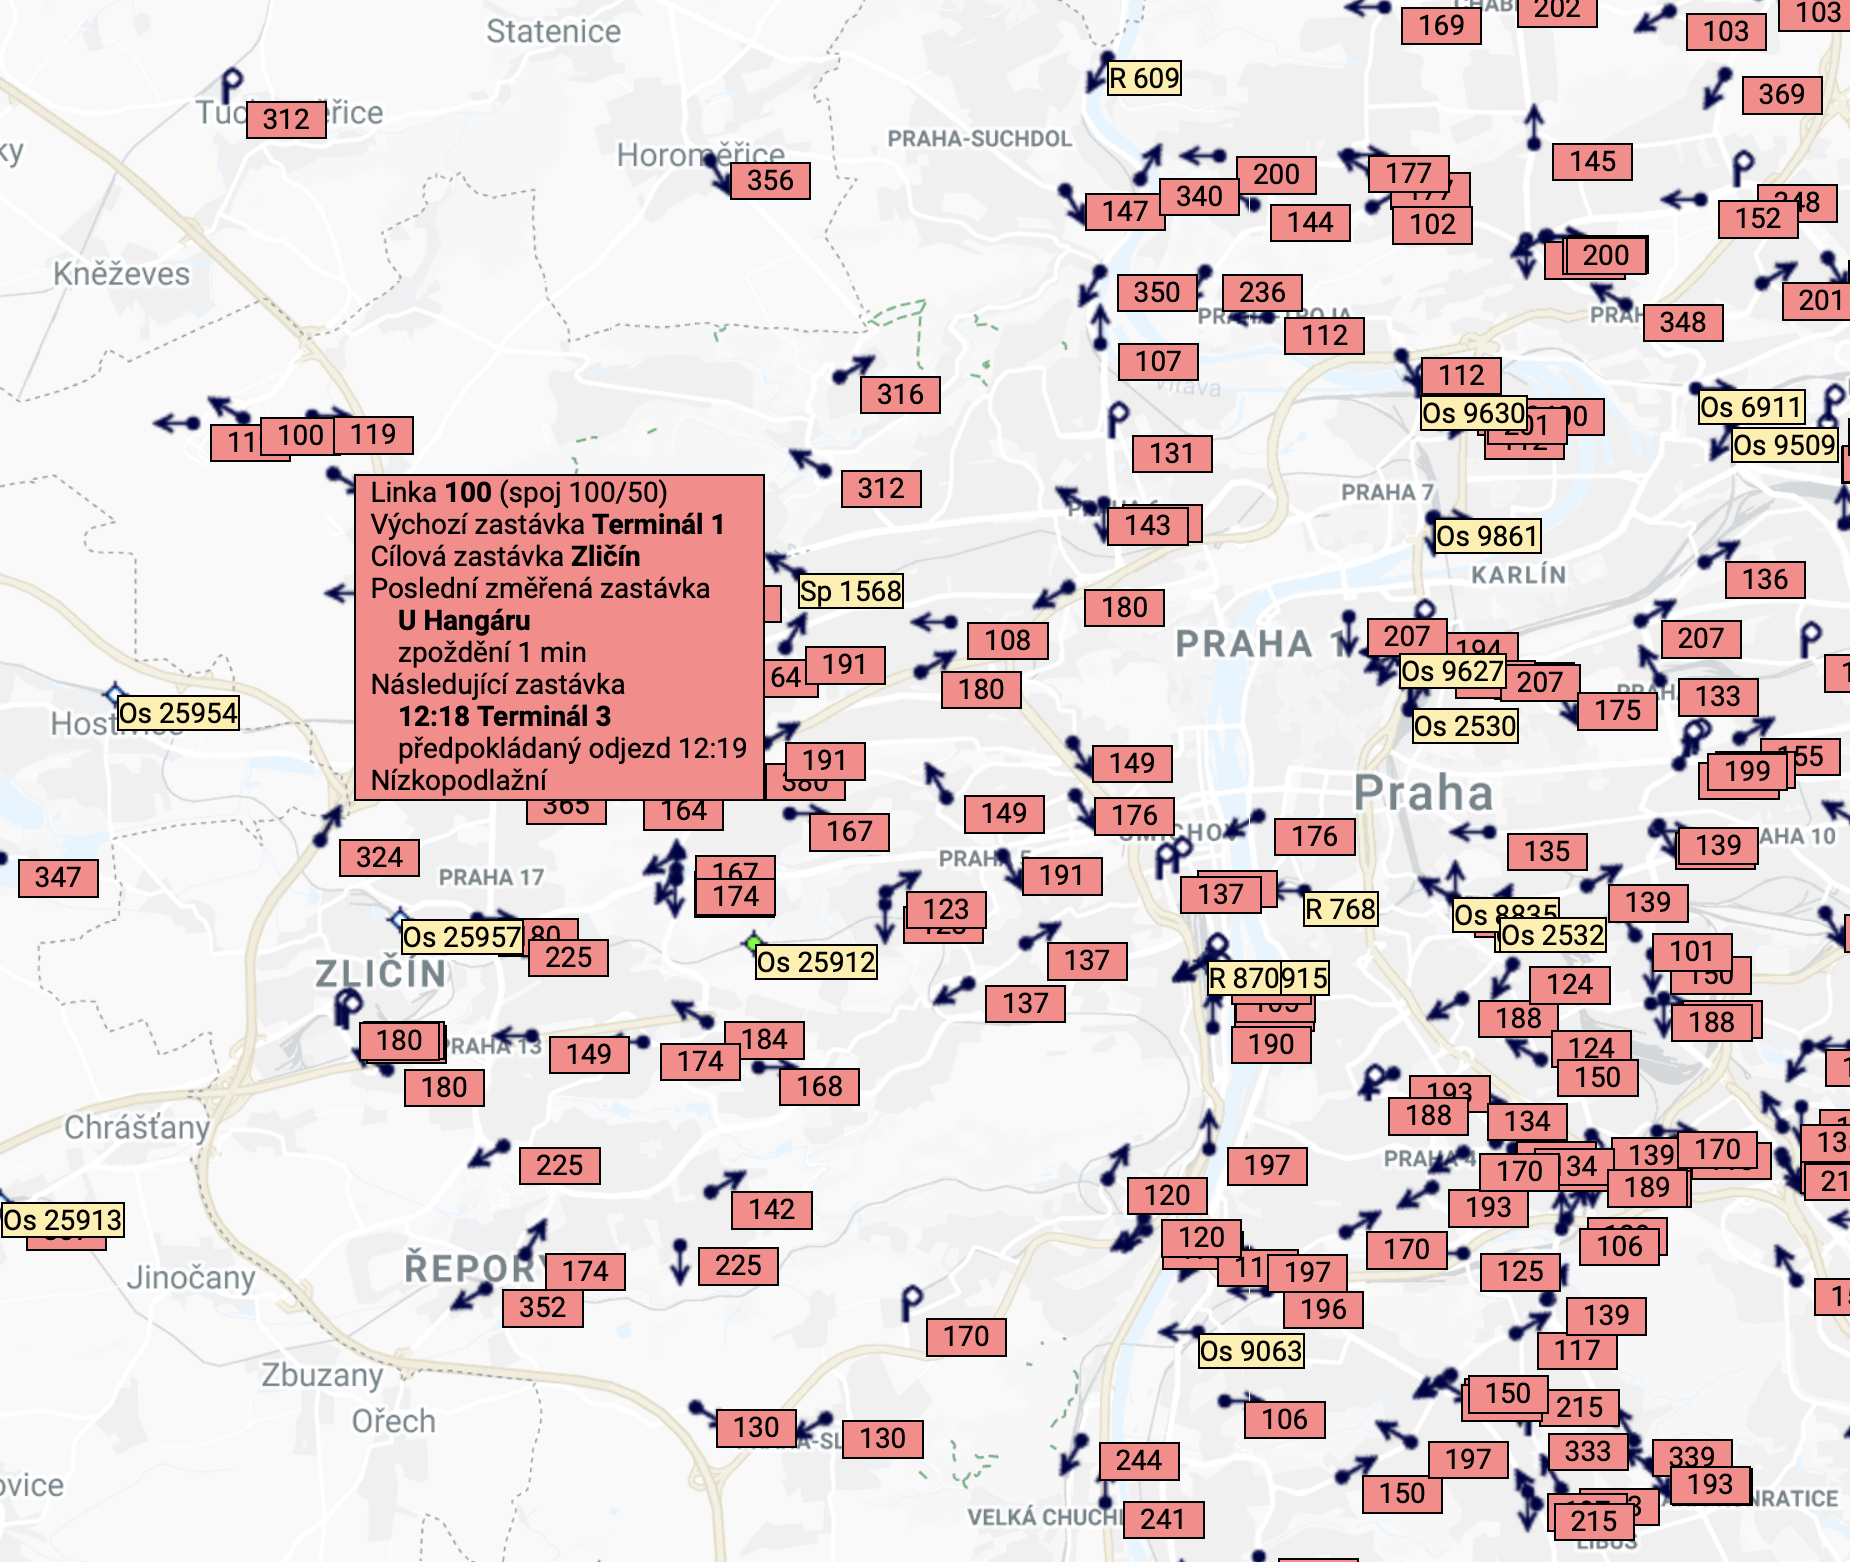
\includegraphics[width=\linewidth]{../img/tram-bus_mapa.png}
  \caption{Mapa z www.tram-bus.cz.}
  \label{fig:tram-bus_result}
\end{figure}

\subsubsection{\gls{idsjmk}}

Mimo Prahu je velice pěkně udělaná aplikace pro zobrazení vozidel \gls{idsjmk} (Integrovaný dopravní systém Jihomoravského kraje). Ten ihned po načtení stránky zobrazuje všechny dobravní prostředky, tedy tramvaje, autobusy a vlaky vše s čísly linek. Dále pak umožňuje po kliknutí na vybraný spoj zobrazit více informací včetně jízdního řádu. Příklad vizualizace je uveden na obrázku \ref{fig:idsjmk_result}.

\bigbreak

Tato aplikace je po vizuální i funkční stránce dobrou inspirací pro tvorbu aplikace v této práci.

\begin{figure}
  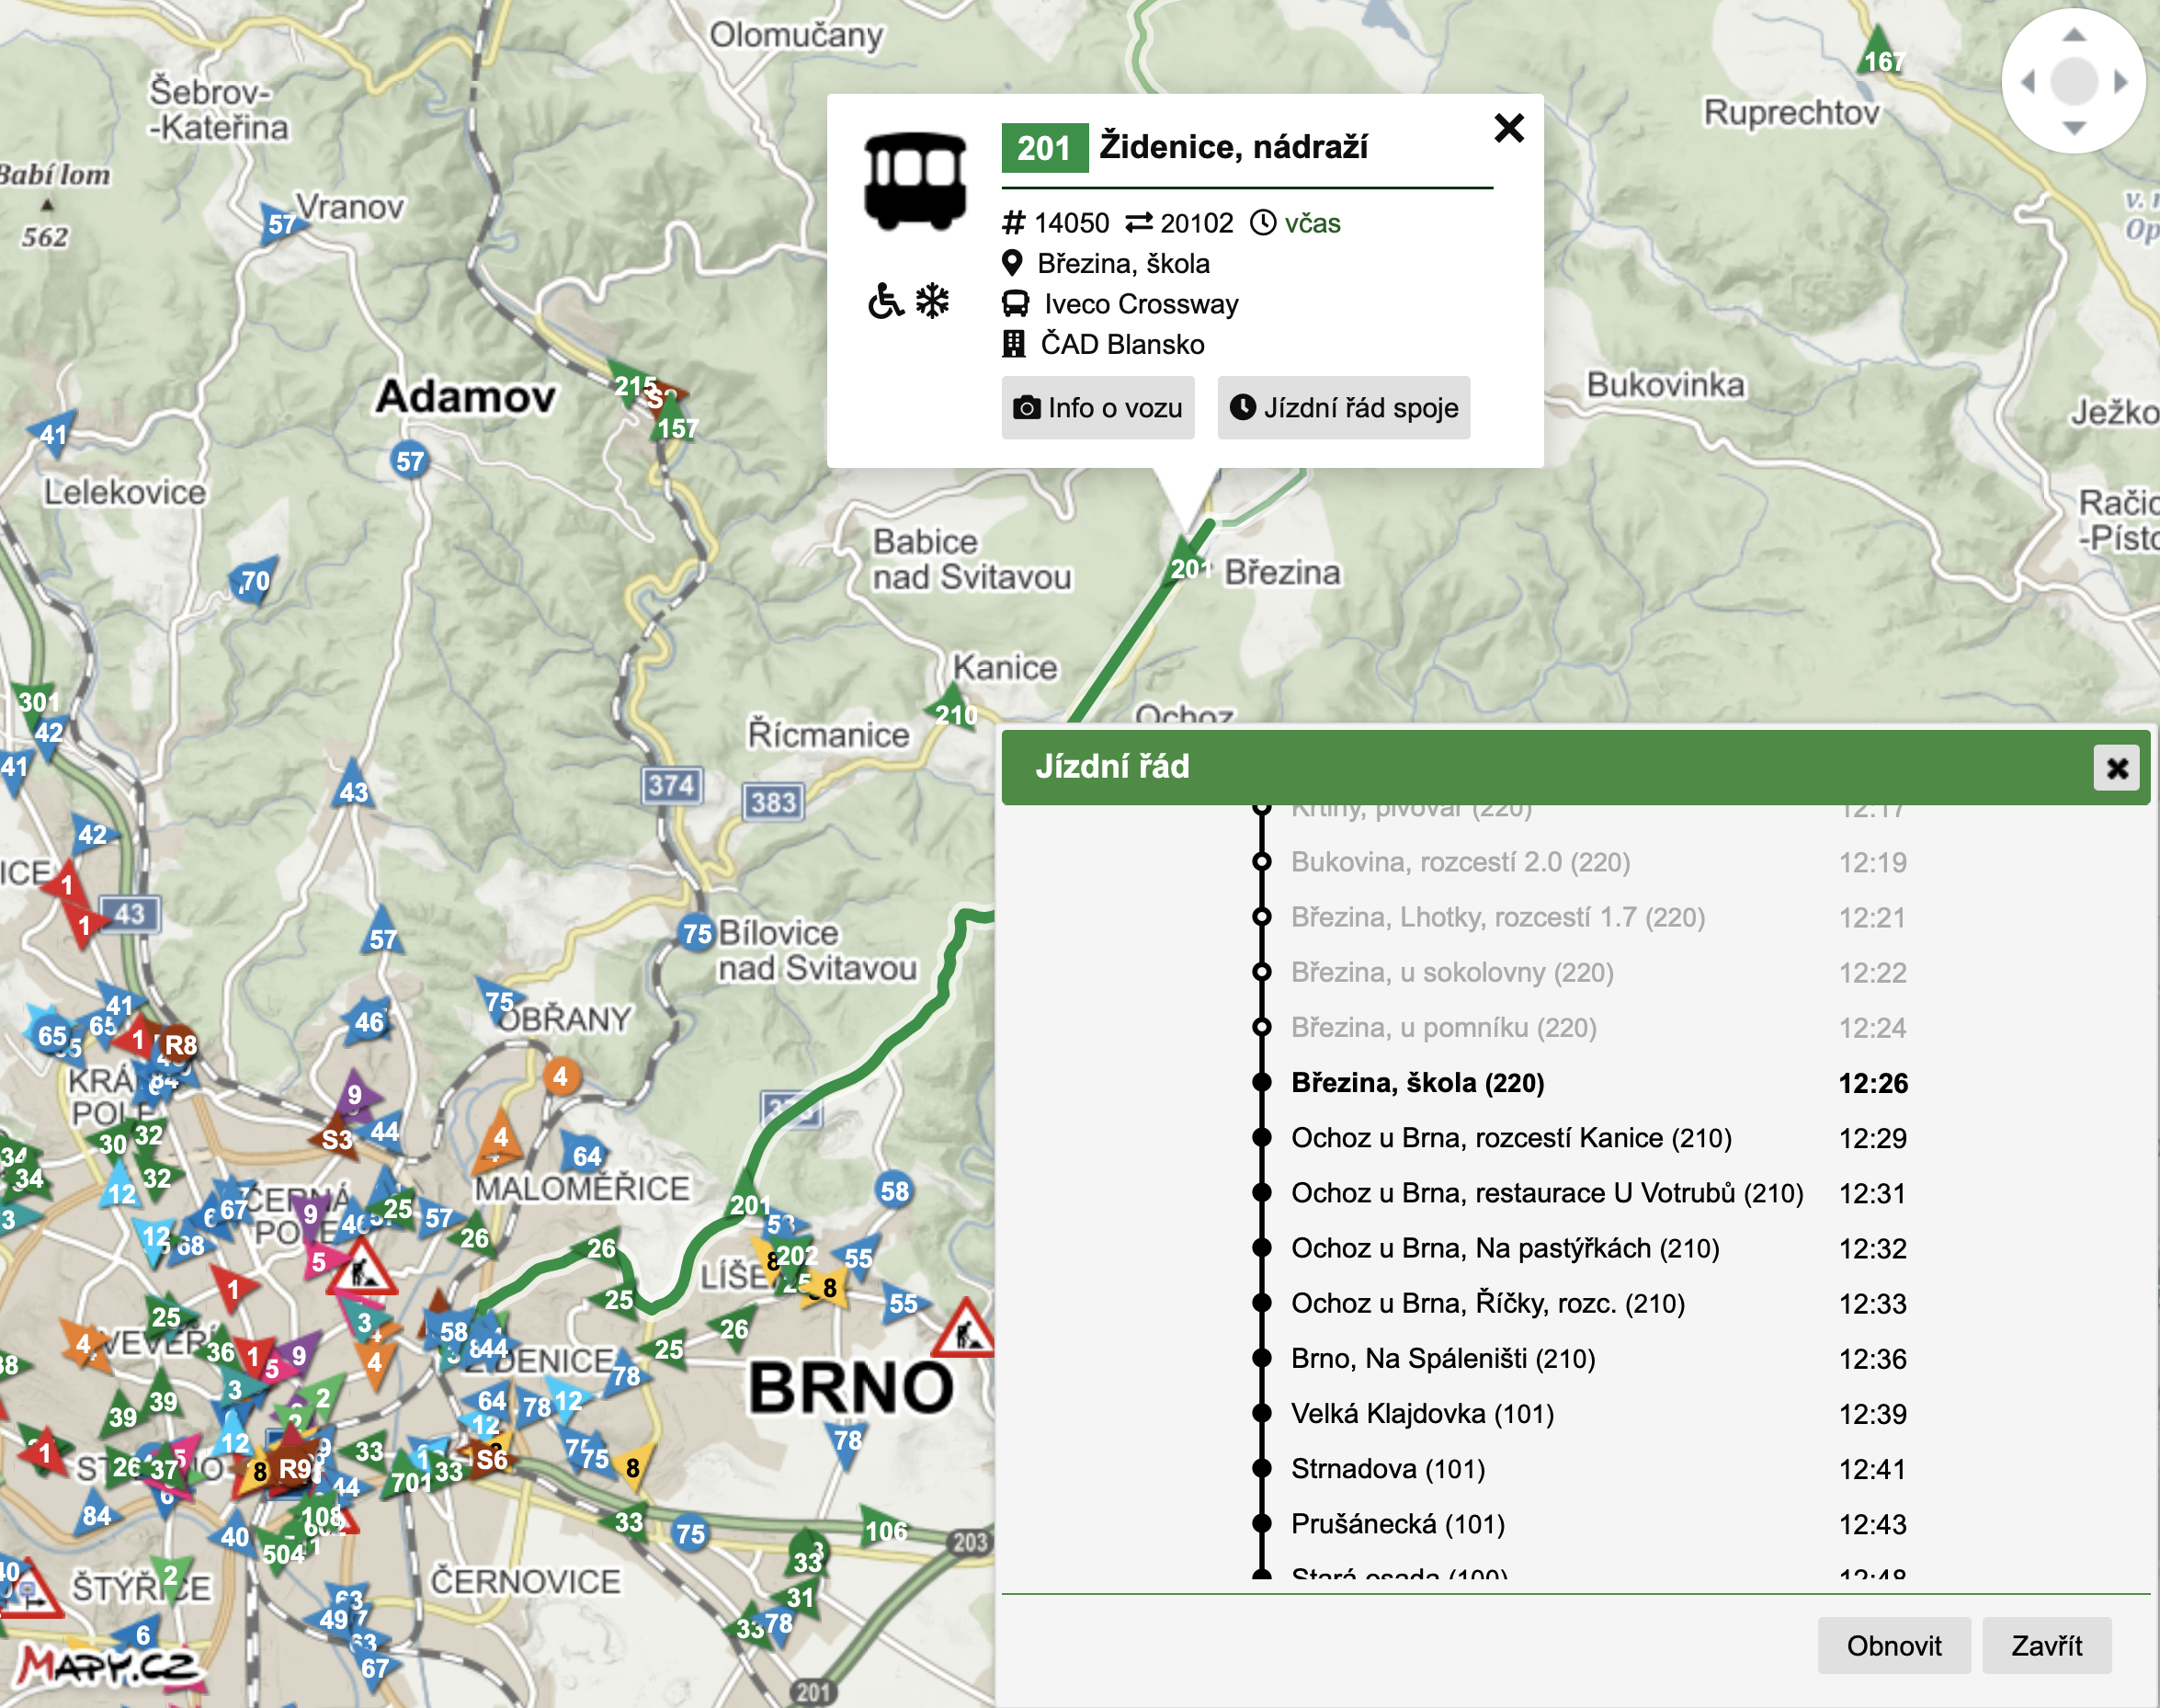
\includegraphics[width=\linewidth]{../img/idsjmk_mapa.png}
  \caption{Mapa z mapa.idsjmk.cz.}
  \label{fig:idsjmk_result}
\end{figure}
